\begin{figure}
	\tikzsetnextfilename{differenziale-totale}
	\centering
	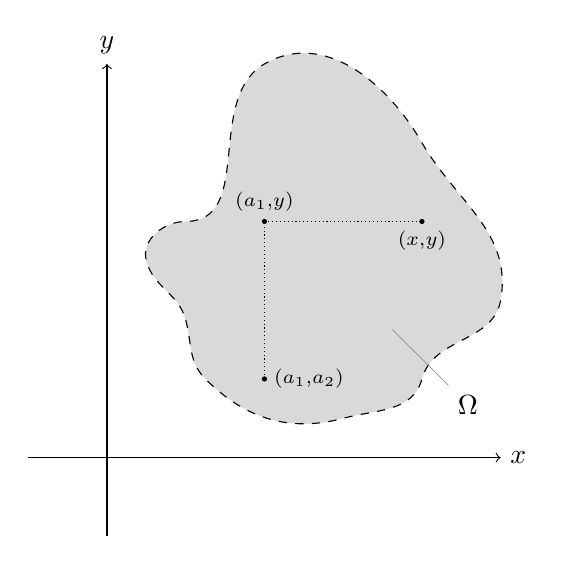
\begin{tikzpicture}
		\draw [black,->] (-1,0) -- (5,0) node[right]{$x$};
		\draw [black,->] (0,-1) -- (0,5) node[above]{$y$};
		\draw [fill=black!15!white,dashed] (1,1.75) to[out=-75,in=135] (1.25,1) to[out=-45,in=195] (3,.5) to[out=15,in=-105] (4,1) to[out=75,in=-100] (5,2) to[out=80,in=-60] (4,4) to[out=120,in=30] (2,5) to[out=210,in=0] (1,3) to[out=180,in=105] (.5,2.5) to[out=-75,in=105] (1,1.75);
		\node [pin={[pin distance=1cm]-45:{$\Omega$}}] at (3.5,1.75) {};
		\draw [densely dotted] (2,1) node[right]{$\scriptstyle(a_1,a_2)$} to (2,3) node[above]{$\scriptstyle(a_1,y)$};
		\draw [densely dotted] (2,3) -- (4,3) node[below]{$\scriptstyle(x,y)$};
		\node [fill=black,circle,scale=.2] at (2,1) {};
		\node [fill=black,circle,scale=.2] at (2,3) {};
		\node [fill=black,circle,scale=.2] at (4,3) {};
	\end{tikzpicture}
	\caption{Incremento $\vec x-\vec a$ scomposto nelle due direzioni lungo gli assi cartesiani in $\R^2$.}
	\label{fig:differenziale_totale}
\end{figure}
